\documentclass{beamer}
\usepackage[utf8]{inputenc}
\usepackage{beamerthemebars}


\usetheme{Madrid}
\usecolortheme{default}

%------------------------------------------------------------
%This block of code defines the information to appear in the
%Title page
\title[] %optional
{Generative Edge Intelligence for IoT-Assisted Vehicle Accident Detection}

\subtitle{Challenges and Prospects}

\author[Angelo Galavotti] % (optional)
{Presented by Angelo Galavotti \\
    Original authors: Jiahui Liu, Yang Liu, Kun Gao, and Liang Wang}

\date[June 2024] % (optional)
{Università di Bologna, June 2024}

%End of title page configuration block
%------------------------------------------------------------



%------------------------------------------------------------
%The next block of commands puts the table of contents at the 
%beginning of each section and highlights the current section:

\begin{document}

%The next statement creates the title page.
\frame{\titlepage}


%---------------------------------------------------------
%This block of code is for the table of contents after
%the title page


\section{Introduction}

%---------------------------------------------------------
%Changing visivility of the text
\begin{frame}
\frametitle{}
As per the World Health Organization's statistics,
vehicle accidents result in over \textbf{1.2 million fatalities annually}.
\begin{itemize}
  \vspace{0.2cm}
  \item To tackle this problem, \textbf{vehicle accident detection} (VAD) is developed to 
  instantly \textbf{transmit} the key \textbf{information of an accident} (i.e., location, possible casualties...) to aid centers.
  \vspace{0.2cm}
  \item VAD relies on \textbf{data processing}, and the \textbf{lack} of vehicle accident \textbf{data} present a \textbf{significant challenge}.
  \vspace{0.2cm}
  \item There's also a need for \textbf{better analysis methods}.
\end{itemize}
\vspace{0.2cm}

\begin{center}
  The solution may lie in the use of \textbf{IoT-assisted} VAD and \textbf{Generative Edge Intelligence}.
\end{center}

\end{frame}


%---------------------------------------------------------

\section{Second section}

%---------------------------------------------------------
%Highlighting text
\begin{frame}
\frametitle{Overview of IoT-assisted VAD}
While conventional VAD requires manual, human investigation of the accident scene, IoT-assisted VAD
makes use of sensors, embedded computers and communication modules.

\begin{itemize}
\item It can rely heavily on the \textbf{cloud} (i.e., for storing data)
\end{itemize}
\end{frame}

\begin{frame}
  \frametitle{Overview of IoT-assisted VAD}
  
  A typical IoT-assisted VAD consists of \textbf{3 phases}:
  \begin{enumerate}
    \item The system uses its onboard \textbf{sensors} to acquire
      \textbf{real-time state data} and sends it to the cloud.
    \item The obtained data
    is then analyzed by \textbf{decision and
    classification algorithms} to determine
    whether an incident has occurred.
    \begin{itemize}
      \item This phase relies on \textbf{cloud} capabilities.
    \end{itemize}
    \item Upon the detection of accidents, an
    \textbf{alert message} is immediately transmitted to emergency services providers.
    \end{enumerate} 

    \begin{figure}[t]
      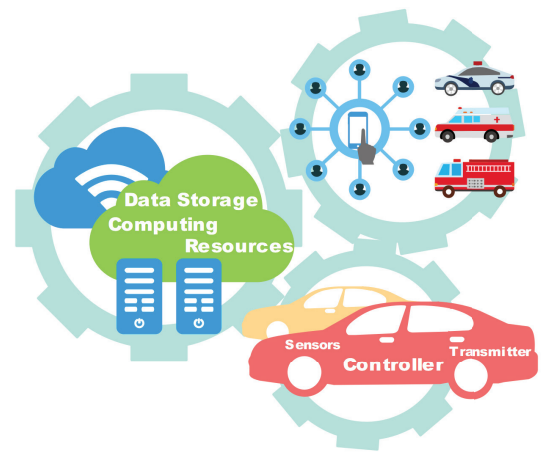
\includegraphics[width=6cm]{images/iot-vad.png}
      \centering
      \end{figure}
\end{frame}


\begin{frame}
  \frametitle{Challenges of IoT-assisted VAD}
  
  \begin{itemize}
    \item \textbf{Accident detection accuracy} which can be compromised due to noisy data from both sensors 
    and wireless communication signals.
    \begin{itemize}
      \item In addition, road conditions and individual driver behavior can lead to
      misjudgments.
    \end{itemize}
    \item \textbf{Accident type classification} (i.e., frontal collision, vehicle fall, roll-over...). This is
    due to data-algorithm barriers.
    \begin{itemize}
      \item There's not enough data or it's not varied enough to train algorithms correctly.
    \end{itemize}
    \item \textbf{Communication performance}: GSM, GPS and other communication technologies frequently used by IoT 
    which can be slow, costly and unreliable.
    \begin{itemize}
      \item Vehicle Ad-hoc Networks (VANETs) lack security, as well as routing
      due to their highly dynamic topology.
    \end{itemize}

  \end{itemize} 
\end{frame}


\begin{frame}
  \frametitle{GEI for VAD}
  
  The application of \textbf{generative models in edge
  computing} is recently gaining attention.
  
  \begin{itemize}
    \item \textbf{Why edge computing?} $\rightarrow$ Allows for fast and low-latency data processing
    at the source of data generation, and reduces the bandwidth.
    \item \textbf{Why generative models?} $\rightarrow$ They capture the underlying intricacies 
    of data, allowing for data augmentation.
    \item \textbf{Why both?} $\rightarrow$ Edge computing satisfies the heavy computational requirements of generative models.  

  \end{itemize}

\end{frame}

\begin{frame}
  \frametitle{Generative Models}
  For \textbf{classification}:
  \begin{itemize}
    \item \textbf{Gaussian Mixture Model
    (GMM)}: it uses multiple Gaussian distributions to
    describe the data distribution.
    \item \textbf{Hidden Markov
    Model (HMM)}: statistical sequence model used for time series data prediction.
  \end{itemize}
  For \textbf{data augmentation}:
  \begin{itemize}
    \item \textbf{Variational Autoencoder (VAE)}: neural network-based generative model that learns a
    \textbf{representation} of input data, allowing it to generate
    new data similar to the input data.
    \item \textbf{Generative Adversarial Network (GAN)}: neural network-based, composed of
    a \textbf{generator} and a \textbf{discriminator}.

  \end{itemize}
\end{frame}


\begin{frame}
  \frametitle{Applications of GEI in VAD}
  \begin{itemize}
    \item \textbf{Data Augmentation}: generation of synthetic data to \textbf{expand} existing
    datasets, and to make it more \textbf{varied}.
    \item \textbf{Accident Classification}: GEI models can discern intricate \textbf{underlying patterns}
     and \textbf{relationships}, improving classification performance.
    \item \textbf{Active Safety Control}: GEI enables
    the \textbf{pre-accident analysis} and the realization
    of active safety control for vehicles. 
    \begin{itemize}
      \item For example, it can generate real-time,
      collision-free trajectories.
    \end{itemize}
  \end{itemize}
\end{frame}

\begin{frame}
  \frametitle{A possible GEI-VAD framework}
  From bottom to top:
  \begin{enumerate}
    \item \textbf{End layer}: includes both vehicles and their sensors,
    as well as \textbf{road infrastructure} (i.e., camera, microwave vehicle detectors).
    \begin{itemize}
      \item Can do a bit of data preprocessing as well.
    \end{itemize}
    \item \textbf{Edge layer}: it nodes for edge computing as well as \textbf{routers} and \textbf{gateways}.
    Generative models are deployed here.
    \begin{itemize}
      \item Also responsible for \textbf{authn/authz} and model selection.
    \end{itemize}
    \item \textbf{Cloud layer}: it possesses high computational power and expansive storage. It's responsible 
    for \textbf{complex model training} as well as \textbf{coordinating} the other layers.
  \end{enumerate}
  \begin{figure}[t]
    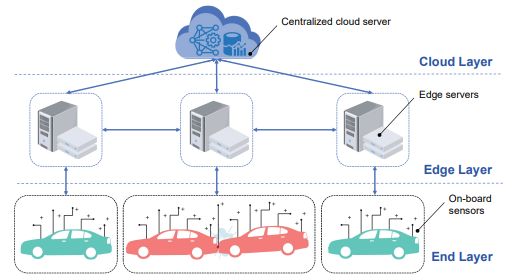
\includegraphics[width=6cm]{images/gei-vad.png}
    \centering
    \end{figure}
\end{frame}

%  future work part
\begin{frame}
  \frametitle{Future directions}
  Some issues in VAD should still be addressed:
  \begin{itemize}
    \item \textbf{Device Compatibility and Interoperability}: to establish
    the end-edge-cloud network architecture, \textbf{standard specifications} 
    and \textbf{protocols} are needed.
    \begin{itemize}
      \item The diversity of
      hardware and software in the IoT networks poses challenges to the 
      deployment of GEI applications.
    \end{itemize}
    \item \textbf{Data Encryption}: VAD systems utilize
    \textbf{sensitive health data}. Therefore,
    \textbf{encryption} is necessary in the architecture to prevent data
    leakage.
    \begin{itemize}
      \item Encryption algorithms should be applied in both storage and data transmission.
    \end{itemize}
  \end{itemize}
\end{frame}

\begin{frame}
  \frametitle{Future directions}
  Some issues in VAD should still be addressed:
  \begin{itemize}
    \item \textbf{Generative Model Interpretability}: enhancing the transparency 
    and interpretability of generative models can increase \textbf{user trust}
    in the GEI-VAD system and aid in its supervision and
    management.
    \item \textbf{Communication Framework}: a \textbf{V2X communication
    architecture} suitable for VAD may improve
    performance in terms of bandwidth, packet transmission delay and packet loss.
  \end{itemize}
\end{frame}

%---------------------------------------------------------

\begin{frame}
  \frametitle{In conclusion}
  The integration of GEI technology can significantly enhance
  the performance of VAD in terms of \textbf{timeliness}, \textbf{accuracy}, and
  \textbf{stability}, thereby contributing to \textbf{improved road traffic safety}.
\end{frame}
%---------------------------------------------------------
\begin{frame}

  \begin{figure}[t]
    
\includegraphics[width=8cm]{images/ending.png}
    \centering
    \end{figure}

    \vspace{0.2cm}


  \begin{center}
    \begin{Large}
      Thank you!
    \end{Large}
  \end{center}
    
\end{frame}
%---------------------------------------------------------


\end{document}